% !TeX spellcheck = english
% !TEX root = thesis.tex
\section{\hlr{Fabrication of crystalline silicon nanoparticles by femtosecond laser ablation}}
\label{sec:Ablation}
        The first part of the project was to develop a new, simple, method of fabricating crystalline dielectric
    nanoparticles. The idea was to use controlled laser ablation~--- a very simple technique~--- to produce the particles.
    Previous work on the topic\cite{kuznetsov2012magnetic, zywietz2014laser} has shown that it is possible to fabricate single particles
    of a certain size.

        We ended up developing two different methods to fabricate crystalline nanoparticles~--- direct laser writing of crystalline
    nanoparticles out of a thin film of amorphous silicon (adapted from a method used for plasmonic nanoparticles\cite{makarov2016controllable,
    dmitriev2016direct}), and a forward transfer of nanoparticles by single femtosecond laser pulses
    from a transparent substrate with a a thin film of amorphous silicon to an arbitrary acceptor substrate. The second method is
    similar to the the one presented in \cite{zywietz2014laser}, but doesn't require any additional annealing steps to achieve
    nanoparticle crystallinity and isn't limited to transparent acceptor substrates.

    \begin{figure}[h!]
            \begin{center}
                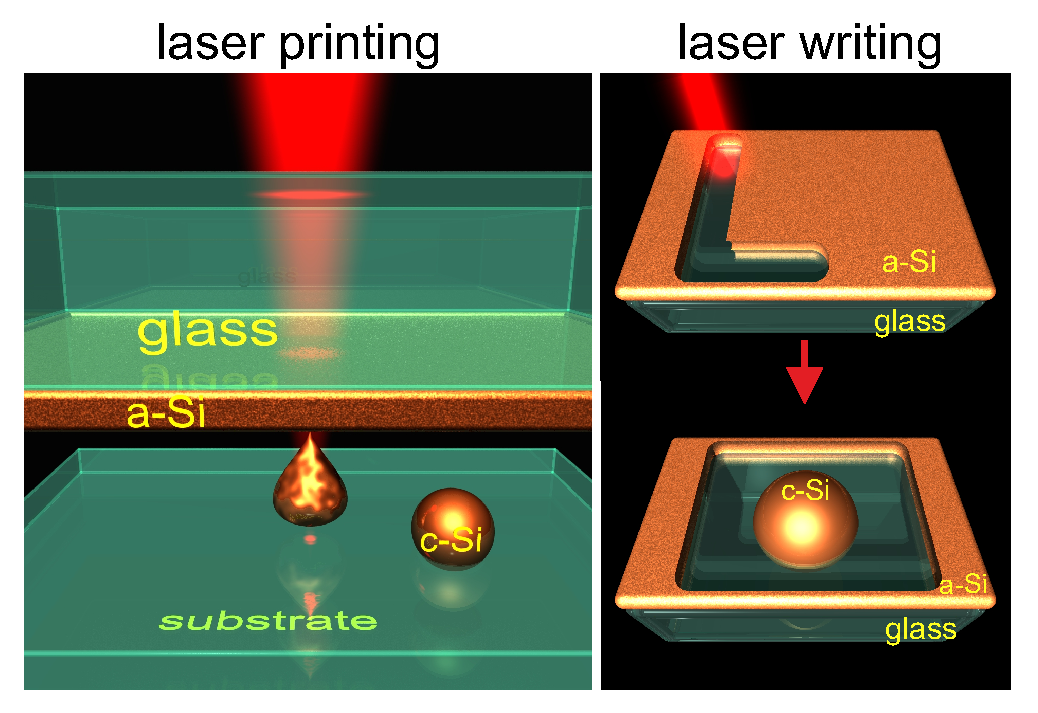
\includegraphics[width=0.5\textwidth]{figs/methods/LaserPrinting.eps}
            \end{center}
            \caption{Geometry of laser-ablation based fabrication methods of crystalline nanoparticles from amorphous
                        thin films.}
            \label{fig:LaserPrinting}
    \end{figure}

    \subsection{\hlr{Generation of femtosecond laser pulses}}

    \subsection{\hlr{Ultrashort-pulse laser albation}}

    \subsection{\hlb{Laser transfer of crystalline dielectric particles}}
            Laser transfer of crystalline nanoparticles was carried out using a femtosecond laser system
        (Femtosecond Oscillator TiF-100F, Avesta Poject), emitting laser pulses at a central wavelength of $800~\si{nm}$,
        with pulse duration of $100~\si{fs}$, and repetition frequency of $80~\si{MHz}$. Single laser pulses were selected
        by a Pockels cell-based pulse picker (also Avesta Project), focused by an oil immersion microscope objective (Olympus $100\times$)
        with a numerical aperture of $\mathit{NA}=1.4$. According to the relation $\emph{d}\approx 1.22\lambda/\mathit{NA}$, the estimated
        diameter of the beam's focal spot size was $d=0.7~\si{\upmu m}$, which was close to the value measured by a method based on
        the dependence of the laser-damaged area on incident laser energy ($0.68~\si{\upmu m}$)~\cite{liu1982simple}.
        The nanoparticles were fabricated from an $80~\si{nm}$ thick a-Si:H film deposited on a fused silica substrate by
        plasma enhanced chemical vapor deposition from a SiH$_{3}$ precursor gas.

            The nanoparticles were fabricated by single laser pulses (from a previously undamaged surface of the a-Si:H film) in a
        forward-transfer geometry, where the receiving substrate is placed under the film with a spacing
        of $\sim 50~\si{\upmu m}$ (figure~\ref{fig:LaserPrinting}(a)). This geometry has an advantage over the back-transfer geometry
        used in \cite{zywietz2014laser}, because of the possibility of transferign nanoparticles onto a wide variety of substrates,
        including opaque and structured samples.

            The silicon nanoparticles were printed at laser energies in the range of $0.5-1.2~\si{nJ}$, providing fluencies in
        the range of $0.12-0.16~\si{J/cm^{2}}$. The fabricated nanoparticles were almost spherical in shape(figure~\ref{fig:Crystallinity}(b))
        and their diameters lie in the range of $50-200~\si{nm}$, depending on the fluence.

    \subsection{\hlb{Laser writing of dielectric particles}}
            The direct laser writing of crystalline Si nanoparticles was carried out from an initially amorphous a-Si:H film.
        The process consists of using a train of femtosecond pulses to cut patches out of the a-Si thin film\cite{makarov2016controllable,
        dmitriev2016direct}. A laser fluence $F\approx100~\si{mJ/cm^{2}}$ provides film heating close to the melting point even in a
        single shot regime, while a pulse train with a $12.5~\si{ns}$ delay between pulses leads to the temperature accumulation
        and exceeding of the ablation threshold. The heat transferring from the ablated area to the surrounding film is accumulated
        much stronger in the cut patches, which are thermally isolated from the rest of the film.
        These micro-patches are unstable at high temperatures and undergo dewetting to a certain number of similar
        nanoparticles~\cite{thompson2012solid}.


\clearpage
